\chapter{\IfLanguageName{dutch}{Stand van zaken}{State of the art}}%
\label{ch:stand-van-zaken}

% Tip: Begin elk hoofdstuk met een paragraaf inleiding die beschrijft hoe
% dit hoofdstuk past binnen het geheel van de bachelorproef. Geef in het
% bijzonder aan wat de link is met het vorige en volgende hoofdstuk.

% Pas na deze inleidende paragraaf komt de eerste sectiehoofding.

% Dit hoofdstuk bevat je literatuurstudie. De inhoud gaat verder op de inleiding, maar zal het onderwerp van de bachelorproef *diepgaand* uitspitten. De bedoeling is dat de lezer na lezing van dit hoofdstuk helemaal op de hoogte is van de huidige stand van zaken (state-of-the-art) in het onderzoeksdomein. Iemand die niet vertrouwd is met het onderwerp, weet nu voldoende om de rest van het verhaal te kunnen volgen, zonder dat die er nog andere informatie moet over opzoeken \autocite{Pollefliet2011}.

% Je verwijst bij elke bewering die je doet, vakterm die je introduceert, enz.\ naar je bronnen. In \LaTeX{} kan dat met het commando \texttt{$\backslash${textcite\{\}}} of \texttt{$\backslash${autocite\{\}}}. Als argument van het commando geef je de ``sleutel'' van een ``record'' in een bibliografische databank in het Bib\LaTeX{}-formaat (een tekstbestand). Als je expliciet naar de auteur verwijst in de zin (narratieve referentie), gebruik je \texttt{$\backslash${}textcite\{\}}. Soms is de auteursnaam niet expliciet een onderdeel van de zin, dan gebruik je \texttt{$\backslash${}autocite\{\}} (referentie tussen haakjes). Dit gebruik je bv.~bij een citaat, of om in het bijschrift van een overgenomen afbeelding, broncode, tabel, enz. te verwijzen naar de bron. In de volgende paragraaf een voorbeeld van elk.

% \textcite{Knuth1998} schreef een van de standaardwerken over sorteer- en zoekalgoritmen. Experten zijn het erover eens dat cloud computing een interessante opportuniteit vormen, zowel voor gebruikers als voor dienstverleners op vlak van informatietechnologie~\autocite{Creeger2009}.

% Let er ook op: het \texttt{cite}-commando voor de punt, dus binnen de zin. Je verwijst meteen naar een bron in de eerste zin die erop gebaseerd is, dus niet pas op het einde van een paragraaf.

% TODO: dit snap ik echt niet?
Deze paragraaf beschrijft de huidige kennis die er bestaat rond dit onderwerp. Eerst zal het belang van beweging gekaderd worden, waarna een link gelegd zal worden naar de invloed die het heeft op mentale gezondheid en de huidige toestand besproken wordt. Daarna zal gamification zeer uitvoerig geanalyseerd worden, waarna ten slotte een blik zal geworpen worden op bestaande sportapplicaties.

\section{Belang van beweging}

\subsection{Gevolgen van een sedentaire levensstijl}
Bij volwassenen wordt een sedentaire levensstijl geassocieerd met schadelijke gevolgen voor de volgende gezondheidskwesties: sterfte in het algemeen, door hart- en vaatziekten en door kanker. \autocite{Bull2020}. Bovendien wordt het ook gelinkt aan het optreden van hart- en vaatziekten, diabetes type 2 en kanker. \textcite{Stanton2020} koppelen verminderde fysieke activiteit ook aan meer depressie-, angst- en stresssymptomen.

Om de kans hierop te verkleinen moeten volwassenen, tussen de 18 en 64 jaar oud, volgens de ``World Health Organization'' (WHO) wekelijks 150 à 300 minuten sporten met gemiddelde intensiteit of 75 à 150 minuten met krachtige intensiteit \autocite{Bull2020}. Voor mensen met een beperking worden dezelfde hoeveelheden sport aangeraden, hoewel daar mogelijks samen met een medisch verantwoordelijke bekeken moet worden in welke mate dit mogelijk is, afhankelijk van de beperking. Voor zwangere of net bevallen vrouwen wordt er minstens 150 minuten per week, met gemiddelde intensiteit, aangeraden. In het algemeen kan dus gesteld worden dat voor elk individu, ongeacht de leeftijd, een bepaalde minimum hoeveelheid beweging aangeraden wordt.

\begin{figure}[h]
    \caption[Fysieke inactiviteit bij volwassenen wereldwijd]{Fysieke inactiviteit volwassenen (15+) wereldwijd, bij mannen (A) en vrouwen (B) \autocite{Bull2020}}
    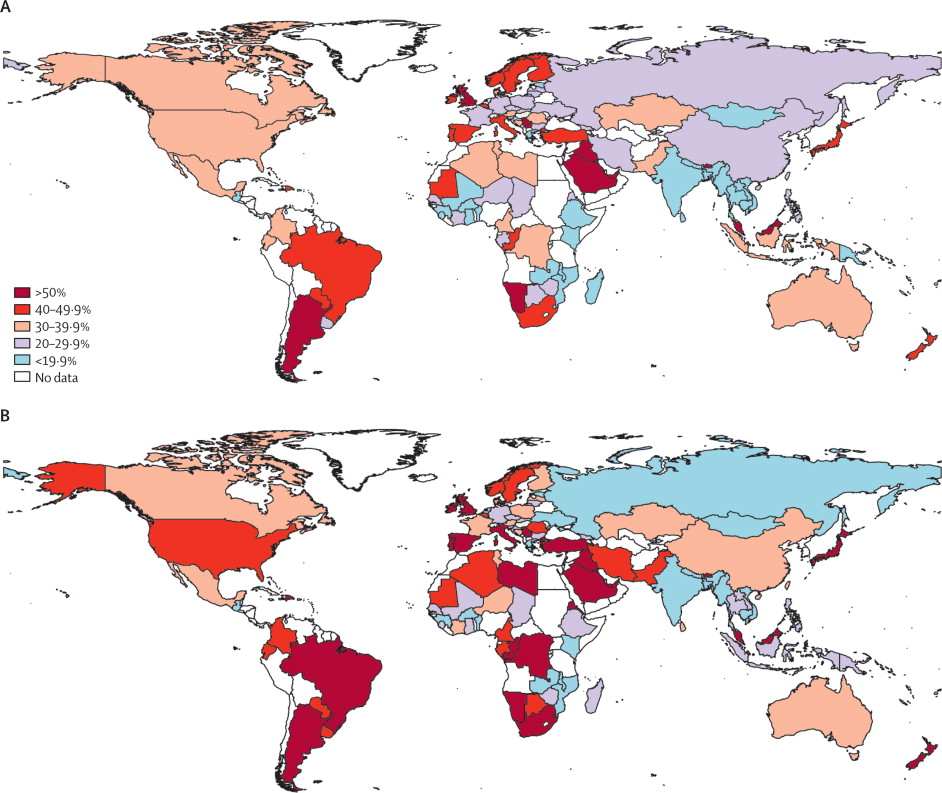
\includegraphics[width=0.5\textwidth]{Inactiviteit}
    \label{fig:inactivity}
\end{figure}

\textcite{Hallal2012} beschouwen 31,1\% van de wereldwijde bevolking als inactief. Dit wil zeggen dat, op het moment van onderzoek, bijna een derde van de volwassen wereldbevolking de vooropgestelde aanbevelingen van WHO, beschreven door \textcite{Bull2020}, niet haalt. Voor Europa ligt deze waarde zelfs op 34,8\% en zoals op Figuur \ref{fig:inactivity} te zien is, ligt België nog een stuk boven de gemiddelde Europese waarde met 40\% à 49,9\%.

\subsection{Invloed van beweging op mentale gezondheid}
Vele studies hebben aangetoond dat er endogene opioïden aangemaakt worden bij het sporten \autocite{Harber1984}. Endogene opioïden (endorfines, enkefalines en dynorfines) zijn peptiden die biochemische eigenschappen hebben die lijken op opiaten zoals heroïne en morfine. Vooral endorfine als gevolg van training wordt in verband gebracht met zowel fysiologische als psychologische veranderingen \autocite{Dishman2009}.

Deze chemische stoffen komen soms vrij als reactie van het menselijk lichaam op pijn, wat ervoor zorgt dat de pijnperceptie kan veranderen \autocite{Chaudhry2023, Dishman2009}. Daarnaast werden ze ook al geassocieerd met een toestand van plezier \autocite{Chaudhry2023}.

Daarnaast stellen \textcite{Mahindru2023} dat voldoende lichaamsbeweging kan helpen met het verbeteren van slaap, wat op zijn beurt zorgt voor het reguleren van normale hormonale en metabolische processen \autocite{Dolezal2017}. Te weinig slapen heeft zelfs een negatieve impact op de economie: het kost Amerikaanse bedrijven en gezondheidszorginstanties jaarlijks miljarden dollars \autocite{Dolezal2017}.


\section{Beweging en productiviteit}
% TODO: meer bronnen, meer cijfers
Wanneer de algemene gezondheid van werknemers slecht is, brengt dit kosten mee voor het bedrijf. \textcite{Sjoegaard2016} beschrijven hoe deze kosten gerelateerd zijn aan de mentale en fysieke afwezigheid van werknemers tijdens het werk, met een verminderde productiviteit tot gevolg. Echter, voor personen die sedentair werk uitvoeren en voornamelijk aan een computer werken, zorgt een verhoogde hoeveelheid sport tijdens de vrije tijd voor minder stres en meer energie op de werkvloer \autocite{Hansen2009}.

Op die manier leidt het invoeren van regelmatige beweging, door middel van op voorhand opgestelde oefeningen en een zorgvuldige begeleiding, volgens \textcite{Cancelliere2011} tot een positief effect op de productiviteit. In die mate dat \textcite{Sjoegaard2016} stellen dat dit effect de eventuele uitgaven in verband met sportactiviteiten overstijgt.



\section{Gamification}
Volgens \textcite{Deterding2011} is gamification te beschrijven als het gebruiken van speldesignelementen in een niet-spelgerelateerde context. Gamification bestaat uit drie hoofdonderdelen: de gebruikte techniek, de psychologische uitkomsten en de verdere invloed op het gedrag \autocite{Hamari2014}. Daarnaast zijn sociale aspecten ook essentieel: door het ontstaan van een competitie streven mensen ernaar erkenning te ontvangen \autocite{Hamari2013}.

\subsection{Meest gebruikte technieken}
% TODO: meer uitwerken en linken leggen naar deze casus
\subsubsection{Punten en scoreborden}
Volgens \textcite{Hamari2014} zijn punten en scoreborden de meest voorkomende technieken. Punten worden toegekend voor het uitvoeren van vooropgestelde taken en aan de hand van deze punten kunnen scoreborden worden opgesteld. Deze scoreborden kunnen de resultaten van meerdere gebruikers tegen elkaar opzetten, wat voor een onderlinge competitie zorgt.

\subsubsection{Uitdagingen}


\subsubsection{Badges}

\subsubsection{Levels}

\subsubsection{Beloningen}


\textcite{Hamari2014} somt punten, scoreborden en vooropgestelde uitdagingen op als de drie meest voorkomende technieken. Daarnaast komen ook volgende methodes veelvuldig voor: het gebruik van levels, en eventueel een daarbij horend verhaal, beloningen, een overzicht van vooruitgang of het bekomen van badges, die bijvoorbeeld de beste gebruiker in een bepaalde categorie aanduiden \autocite{Dong2012,Flatla2011,Li2012}.
Daarbij kunnen de gehanteerde technieken verder ingevuld worden naar wens. Zo kunnen beloningen bijvoorbeeld bestaan uit, maar daarom niet gelimiteerd worden tot, een donatie aan een gekozen goed doel of een eervolle vermelding op een intern bedrijfsevenement.

\subsection{Psychologische aspecten}
% TODO: terugkoppelen naar technieken
Gamification is sterk gebaseerd op psychologie. Wanneer psychologische aspecten bevraagd zijn, is er vooral gefocust op motivatie, attitude en plezier \autocite{Hamari2014}. \textcite{Cheong2013} werkte een online quiz uit die gamification gebruikt, met als doel om studeren aan te moedigen door het leuker te maken. Uit een bevraging  na de quiz bleek dat 40,79\% van de deelnemers enthousiast en 46,05\% van de deelnemers tevreden was tijdens de quiz. Daarenboven was het merendeel (77,63\%) van de deelnemers voldoende gemotiveerd om de quiz te vervolledigen.

\subsection{Invloed op gedrag}
\textcite{Kari2016} stellen dat gamification in sportapplicaties een positieve invloed heeft op de intrinsieke bewegingsmotivatie, wat ervoor zorgt dat gebruikers gaan handelen naar een bepaald doelgedrag. \textcite{PoloPena2020} bevestigen dit, maar voegen hier wel aan toe dat gamification een grotere invloed heeft op vrouwen dan op mannen, en op oudere mensen dan op jongere gebruikers. % TODO: WAAROM?

Studies van \textcite{Hamari2013a} hebben aangetoond dat de resultaten van gamification mogelijks niet voor alle gebruikers op lange termijn doeltreffend zijn, en de invoering ervan mogelijks niet op iedereen het gewenste effect heeft.
Anderzijds zal het verwijderen van spelelementen uit een dienst schadelijke gevolgen hebben voor de gebruikers die wel nog betrokken zijn tot het gamification-aspect: zo kan een gebruiker plots al zijn vooruitgang of verdiende badges verliezen.

\subsection{Sociale aspecten}
% TODO: linken met eigen casus
Er zijn twee belangrijke sociale aspecten om in acht te nemen wanneer gamification geïmplementeerd wordt.

Enerzijds is er erkenning, wat beschreven kan worden als de sociale feedback die gebruikers krijgen op hun gedrag \autocite{Cheung2011}.
Wanneer een dienst, zoals het aanbieden van een platform met gamification, erkenning van de andere gebruikers oplevert, wordt die dienst positiever ervaren \autocite{Preece2001}.
\textcite{Hamari2013} suggereren dat er vervolgens, als gevolg van de ontvangen erkenning, een bepaalde bereidheid ontstaat om de erkenning wederkerig te maken. Hierdoor zal de tegenpartij ook op zijn beurt de dienst positiever ervaren.

Anderzijds is er sociale invloed, wat verwijst naar de perceptie van een individu over het belang dat anderen hechten aan een bepaald doelgedrag en of ze verwachten dat iemand dat gedrag zal vertonen \autocite{Ajzen1991}. Specifiek voor een platform dat gamification implementeert, kan er sociale invloed ontstaan door het zien van wat andere gebruikers op het platform presteren. Hierdoor wordt namelijk een verwachtingspatroon gecreëerd en zetten gebruikers elkaar aan tot het behalen van een bepaald doelgedrag, zoals vaker sporten.

\section{Bestaande sportapplicaties}
Hieronder volgt een diverse greep uit de bestaande mobiele en desktop sportapplicaties en -platformen en welke spelelementen daarin gebruikt worden.

\href{https://www.strava.com/}{Strava} is een applicatie waarmee gebruikers hun sportprestaties kunnen bijhouden. \textcite{Barratt2017} stelt dat deze applicatie gamification toepast in de vorm van uitdagingen en persoonlijke trainingsvooruitgang.

\href{https://www.nike.com/be/en/nrc-app}{Nike Run Club} is een loopapplicatie met meer dan 10 miljoen downloads\footnote{\href{https://bootcamp.uxdesign.cc/how-the-nike-run-club-app-got-runners-hooked-2850c7654fc5}{How the Run Club App got runners hooked - Leevey}} op de Google Play Store en de App Store. Deze applicatie maakt het mogelijk voor lopers om een looptraining vast te leggen, punten te verdienen en andere gebruikers uit te dagen. Daarnaast kunnen ze eigen doelstellingen aanmaken en delen, zodat samen naar een gezamenlijk doel gewerkt kan worden \autocite{StaalnackeLarsson2013}.

Een derde voorbeeld is \href{https://connect.garmin.com/}{Garmin Connect}. Het verschil met de vorige twee applicaties, is dat dit platform enkel voor gebruikers met een Garmin-toestel bedoeld is. Deze applicatie focust vooral op badges \autocite{Ilhan2019}. Het behalen van zulke badge kan dan punten opleveren en de mogelijkheid geven tot het behalen van nieuwe, meer uitdagende badges. Om negatieve gevoelens van frustratie op een mindere dag tegen te gaan, krijgt de gebruiker de optie om andere, niet fysieke activiteiten, uit te voeren om ook dan punten te verdienen.
% TODO: ga ik ook echt meer dan 1 api linken?
Voor deze casus is echter een platform nodig dat aan de hand van de Strava API een competitie opzet die gericht is op mensen in een zittend beroep. Door de focus op deze doelgroep, zullen mensen minder snel gedemotiveerd zijn. Dergelijke applicatie zal ontwikkeld worden in een volgende fase van het onderzoek.
